\documentclass{article}

% ready for submission
\usepackage[preprint]{neurips_2022}

\usepackage[utf8]{inputenc}     % allow utf-8 input
\usepackage[T1]{fontenc}        % use 8-bit T1 fonts
\usepackage{hyperref}           % hyperlinks
\usepackage{url}                % simple URL typesetting
\usepackage{booktabs}           % professional-quality tables
\usepackage{amsfonts}           % blackboard math symbols
\usepackage{amsmath}            % math
\usepackage{nicefrac}           % compact symbols for 1/2, etc.
\usepackage{microtype}          % microtypography
\usepackage{xcolor}             % colors
\usepackage{graphicx}           % figures
\newcommand{\new}[1]{{\color{red} #1}}

\title{TC-DPMixer: A Small, Interpretable Time-Conditioned Mixer for
       Multi-Horizon Energy Forecasting}

\author{%
  Yiyang Chen \\
  Department of Computer Science and Engineering\\
  University of California, Riverside\\
  Riverside, CA 92521 \\
  \texttt{ychen1420@ucr.edu} \\
}

\begin{document}

\maketitle

\begin{abstract}
In modern time-series forecasting architectures, we have seen many powerful architectures that encode different inductive biases.
Combining several opaque forecasting components does not by itself
produce an interpretable model. What can be made readable, even
with opaque components inside, is the rule that decides how much
weight each component carries. We use this observation to build
\emph{TC-DPMixer}, a four-branch additive mixer for appliance-load
forecasting in which the combination weights are emitted by a small
MLP that reads only the calendar feature vector. The branches are
the usual ones --- persistence anchor, target decomposition, channel
mixer, time mixer --- and the gate is the only part of the network
the reader is asked to inspect. Its 24-hour schedule is a
deterministic function of clock time and is plotted directly. Five seeds put TC-DPMixer at
$214.44 \pm 0.75$\,Wh/h on the weekly task against iTransformer's
$219.91 \pm 2.42$, with a 187K parameter count against 440K and a
$3\times$ lower training time; the paired difference is $5.47$\,Wh/h,
the 95\,\% bootstrap CI is $[-6.93, -4.11]$, and the paired Cohen's
$d$ is $2.87$. Reducing the backbone to a persistence anchor, the
time-mixer branch, and the calendar gate gives a 116K-parameter
model at $211.73 \pm 0.92$\,Wh/h. The gate output is a fixed
function of clock time, so its 24-hour schedule is directly
visualisable and unaffected by weather perturbations. The short
horizon trades the other way: iTransformer leads at $34.15 \pm 0.48$
\,Wh, with TC-DPMixer 0.84 behind. This is one dataset, one
household, one CS\,228 final project; cross-house transfer is not
tested. Code:
\href{https://github.com/cyy-07/UCR-CS228-Project}{github.com/cyy-07/UCR-CS228-Project}.
\end{abstract}

\section{Introduction}

Time-series forecasting is significant in many tasks, such as modeling human behavior and anomaly detection. In recent years, we have witnessed so many models that are powerful and have achieved strong prediction accuracy on different benchmarks. However, forecasting tasks can vary substantially in their temporal scope, and different horizons may require different predictive mechanisms. For example, redicting the next few hours and predicting the next week are often treated as the same forecasting problem. Short-horizon forecasts often rely heavily on recent observations, while longer horizons may depend more on recurring seasonal and temporal patterns.

To explore energy time-series forecasting, we study the UCI Appliances Energy dataset \citep{candanedo2017}, a 4.5-month single-household energy record sampled every 10 minutes. We consider two forecasting settings: a short-horizon task that predicts the next 4 hours from the previous 16 hours, and a long-horizon task that predicts the next week from the previous week.

In recent years, Transformer-based models such as iTransformer \citep{itransformer} have achieved strong results on many forecasting benchmarks, while some light-weight model like DLinear \citep{dlinear} showed that a much simpler linear architecture can remain highly competitive in some settings. Mixer-style models such as TSMixer \citep{tsmixer} have provided another lightweight alternative by modeling interactions across time and channels through MLP-based components. Meanwhile, routing-based approaches such as Mixture-of-Linear-Experts (MoLE) \citep{mole} suggest that different forecasting mechanisms can be combined dynamically rather than relying on a single predictive pathway. These results suggest that different forecasting mechanisms may be useful for different parts of the prediction problem, motivating the use of input-dependent routing strategies to combine them within a single framework. This motivates the following question:

Can a lightweight forecasting model combine multiple predictive mechanisms while remaining easy to inspect?

To this end, we propose TC-DPMixer, a four-branch additive forecasting model consisting of a persistence anchor, a decomposition branch, a channel-mixing branch, and a time-mixing branch. A small calendar-conditioned gating that determines the relative contribution of each branch throughout the day. Because the gate depends only on calendar features, the resulting routing policy can be visualized directly as a 24-hour schedule.


\textbf{Contributions.}
\begin{itemize}
\item We propose TC-DPMixer, a four-branch additive forecasting model whose routing policy is determined by calendar features alone, allowing the learned 24-hour schedule to be visualized directly.

\item We establish a reproducible benchmark on the UCI Appliances Energy dataset across short- and long-horizon forecasting tasks, including statistical significance tests, block cross-validation, and efficiency analysis.

\item We show that the learned routing policy remains consistent across gate visualization, branch ablation, and a reduced model variant, providing a coherent picture of how the forecasting mechanisms are used on this dataset.
\end{itemize}

\section{Method}
\label{sec:method}

\paragraph{Problem setup.}
A window $x_{1:L}\in\mathbb{R}^{L\times C}$ holds $L$ steps of $C$
channels --- appliance load, lights, room temperatures and humidities,
six outdoor weather variables, and six calendar encodings. The
forecast target $\hat{y}_{L{+}1:L{+}H}\in\mathbb{R}^{H}$ is the
appliance channel; $H\in\{24, 168\}$ controls the short and weekly
horizons. The headline numbers use chronological 70/15/15 splits and
five seeds per configuration; the block-CV runs in
Table~\ref{tab:blockcv} sweep the cut from 55/15/30 to 70/15/15.

\paragraph{Four-branch backbone (DPMixer).}
DPMixer is a weighted sum of four parallel branches:
\begin{equation}
\hat{y}_{t+h}
\;=\; \alpha_{0}\,x_{t,0}
\;+\; \alpha_{1}\,\mathbf{B}_{\text{dec}}
\;+\; \alpha_{2}\,\mathbf{B}_{\text{ch}}
\;+\; \alpha_{3}\,\mathbf{B}_{\text{tm}},
\label{eq:dpmixer}
\end{equation}
The persistence anchor repeats the last observed target value
$x_{t,0}$ across the forecast horizon, corresponding to a simple baseline
that assumes future demand remains close or the same to the most recent observation;
the three learned branches are:
$\mathbf{B}_{\text{dec}}$, a DLinear-style trend $+$ seasonal
decomposition on the target channel \citep{dlinear} (moving-average
kernel 25, two parallel linear heads);
$\mathbf{B}_{\text{ch}}$, two MLP-Mixer blocks acting on the last
timestep across all $C$ channels followed by a linear projection to
$H$; and
$\mathbf{B}_{\text{tm}}$, two MLP-Mixer blocks acting along the time
axis on the target channel followed by a linear projection to $H$
\citep{tsmixer}. Hidden dimensions and dropout are listed in
Appendix~\ref{si:impl}. The gated persistence anchor turns prediction
into residual learning when $\alpha_{0}\approx 1$; without anchoring,
a vanilla MLP on the same window only reaches $R^{2}{=}+0.02$
(Table~\ref{tab:persr2}).

\paragraph{Time-conditioned gating (TC).}
In TC-DPMixer the four branch gates are produced on-the-fly by a
small MLP that reads only the calendar features at the last input
step(which means that we only encode the time), $c_{t}\in\mathbb{R}^{6}$:
\begin{equation}
\alpha_{k}(c_{t})
\;=\; 2\,\sigma\!\big(\mathrm{MLP}_{k}(c_{t})\big)
\;\in\;[0, 2],
\qquad k\in\{0, 1, 2, 3\},
\label{eq:tc}
\end{equation}
where $\mathrm{MLP}$ is a $6\to 16\to 4$ feed-forward network with ReLU
activations and the output layer initialised to zero, so the network
starts with all four branch weights equal to one. The gates are not
constrained to a probability simplex; each can independently amplify
or down-weight its branch in $[0, 2]$. The routing idea follows
Mixture-of-Linear-Experts \citep{mole}; the experts here are
heterogeneous inductive-bias branches rather than copies of the same
linear head in original MoLE paper\citep{mole}. Because $c_{t}$ contains no weather or load history, the
24-hour schedule $\alpha_{k}(\cdot)$ is a fixed function of the
calendar (Figure~\ref{fig:gate}).

\paragraph{Variants.}
SS-DPMixer attaches a NILM-style spike head \citep{nilm}: a smooth
base stream (persistence $+$ DLinear) plus a sigmoid-gated spike
classifier multiplied by a magnitude regressor, both read from the
channel and time MLP-Mixer branches. TC-SS-DPMixer combines the
calendar gate with the spike head. The minimal variant in
Section~\ref{sec:exp} keeps only the persistence anchor, the
time-mixer branch, and the calendar gate.

\paragraph{Training.}
All models use Adam ($\eta{=}10^{-3}$, weight decay $10^{-4}$), $L_{1}$
loss on $\log(1+y)$ targets, batch size 64, early stopping with patience
10, and 5 seeds per configuration. Hyperparameters were tuned on the
validation split only.

\begin{figure}[t]
  \centering
  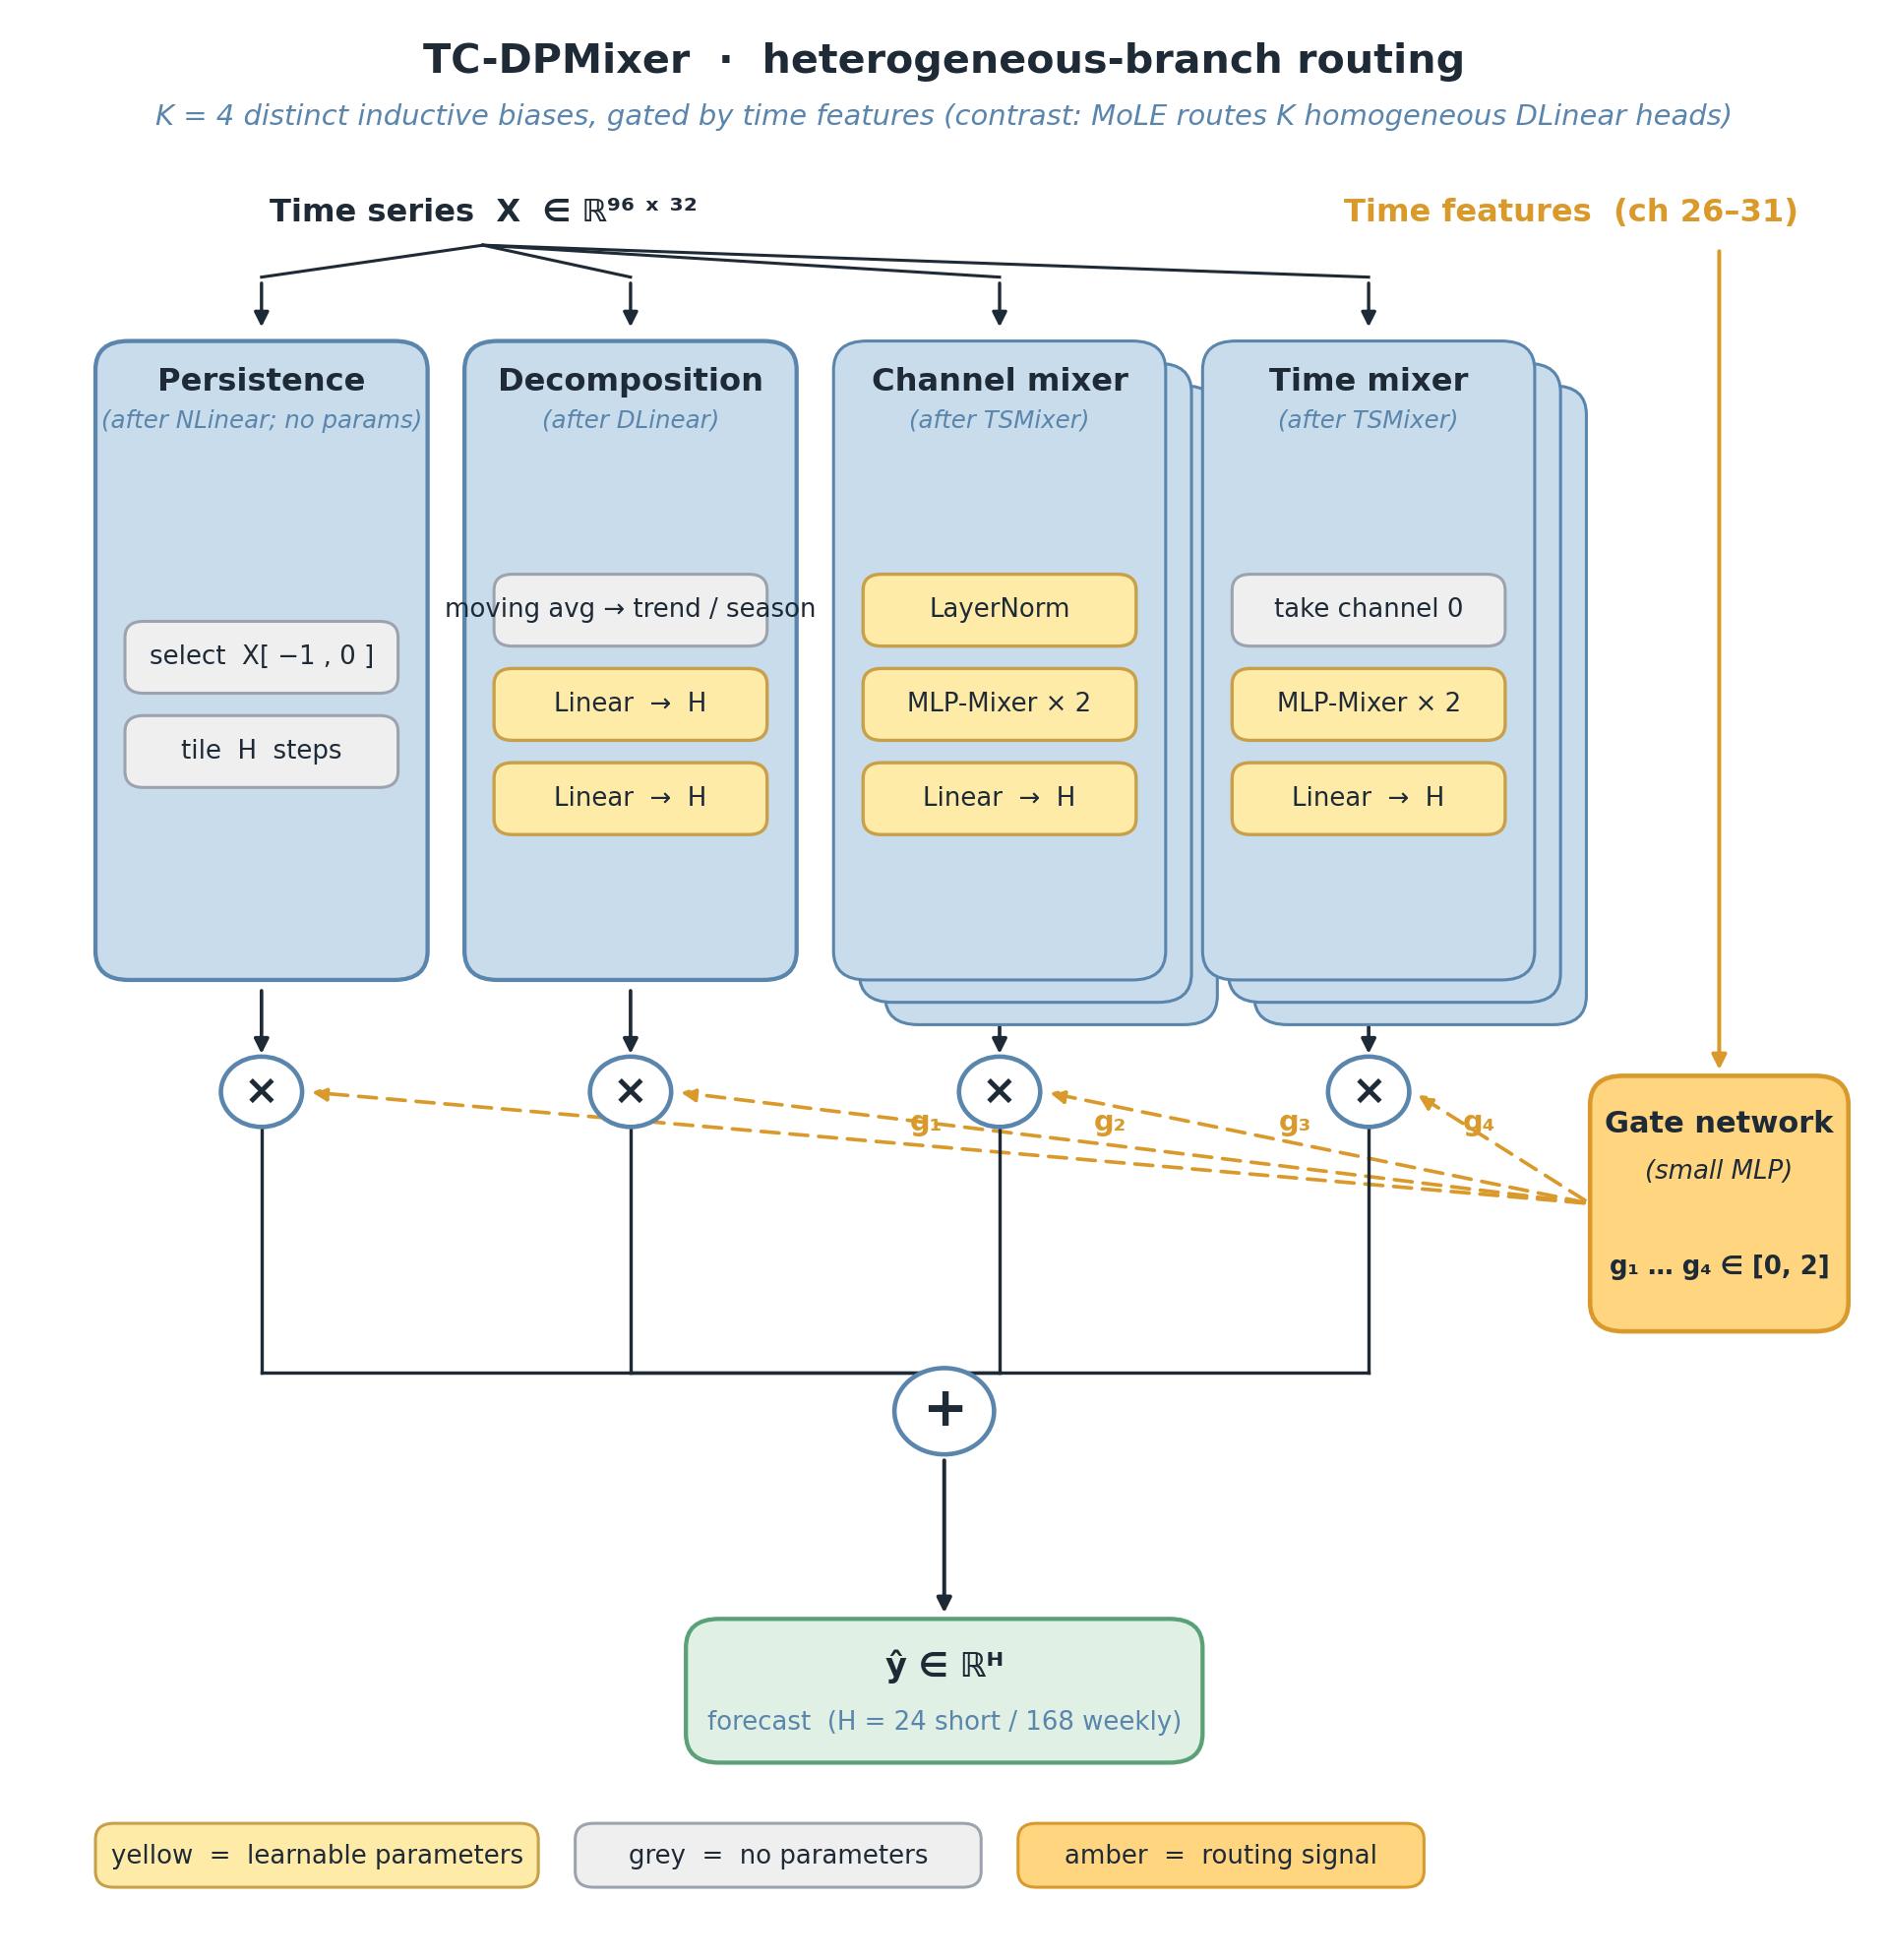
\includegraphics[width=0.95\linewidth]{figures/fig_architecture_mole_style.png}
  \caption{\textbf{TC-DPMixer architecture.} Four parallel branches
    (persistence anchor, target decomposition, channel mixer, time
    mixer) are summed under per-branch gates. A small MLP reads only
    the calendar feature vector $c_{t}$ and outputs four gates
    $\alpha_{k} = 2\,\sigma(\mathrm{MLP}_{k}(c_{t})) \in [0, 2]$; the
    gate has no access to weather or load history, so its 24-hour
    schedule is a deterministic function of clock time.}
  \label{fig:arch}
\end{figure}

\paragraph{Relation to prior work.}
DLinear and NLinear \citep{dlinear}, TSMixer \citep{tsmixer}, TimeMixer
\citep{timemixer}, PatchTST \citep{patchtst}, iTransformer
\citep{itransformer}, N-BEATS \citep{nbeats}, NILM seq2point
\citep{nilm}, and MoLE \citep{mole} are the baselines and design
ancestors of this work. Section~\ref{si:related} in the supplementary
material covers each of them.

\section{Experiments}
\label{sec:exp}

\paragraph{Setup.}
We use the UCI Appliances Energy dataset \citep{candanedo2017} resampled
to 1-hour buckets, with the 4.5-month history split chronologically as
70/15/15. We compare against two non-parametric baselines (Persistence,
Seasonal-Naive) and four learned baselines: DLinear, PatchTST,
iTransformer, and the un-gated DPMixer. We report mean$\pm$std over five
seeds; the weekly headline pair is tested with a paired Wilcoxon
signed-rank test and a paired bootstrap CI (no multiple-comparison
correction is applied; the other contrasts are descriptive).
Short-horizon error is in Wh (MAE over the next 4\,h of hourly output)
and weekly error is in Wh/h (MAE averaged over 168\,h).

\paragraph{Persistence has $R^2 = -0.42$ on the short task.}
Persistence reaches 48.86\,Wh MAE on the short task and looks
acceptable next to learned baselines (Table~\ref{tab:persr2}). Its
$R^{2}$ on the same split is $-0.42$. A constant-mean predictor
would do better, which is why we read the short-task MAE leaderboard
as uninformative and anchor every learned model on the persistence
residual $\hat{y}=x_{t,0}+f(X)$. With that anchor a 4-layer MLP
recovers $R^{2}=+0.12$ at 36.24\,Wh. We read
this as evidence that the short-task MAE leaderboard is uninformative
on its own. Anchoring a small MLP on the persistence residual
$\hat{y}=x_{t,0}+f(X)$ recovers a positive $R^2$ of $+0.12$ at
36.24\,Wh, which is the design we carry forward to every learned
model in this report.

\begin{table}[h]
  \centering
  \caption{Short-horizon ($H{=}24$) diagnostic. Persistence has an
    acceptable MAE but a negative coefficient of determination: the
    constant-mean predictor is strictly better. Anchoring a small MLP on
    persistence ($\hat{y}=x_{t,0}+f(X)$) recovers a positive $R^{2}$.}
  \label{tab:persr2}
  \begin{tabular}{lcc}
    \toprule
    Model & MAE (Wh) $\downarrow$ & $R^{2}$ $\uparrow$ \\
    \midrule
    Persistence       & 48.86 & $-0.42$ \\
    Vanilla MLP       & 39.05 & $+0.02$ \\
    Anchored MLP $(\hat{y}=x_{t,0}+f(X))$ & \textbf{36.24} & \textbf{+0.12} \\
    \bottomrule
  \end{tabular}
\end{table}

\paragraph{TC-DPMixer lowers weekly MAE by 5.47 Wh/h over iTransformer.}
Five seeds put TC-DPMixer at $214.44 \pm 0.75$\,Wh/h on the weekly
task and iTransformer at $219.91 \pm 2.42$
(Table~\ref{tab:headline}). The paired difference is 5.47\,Wh/h, the
95\,\% bootstrap CI is $[-6.93, -4.11]$, and the paired Cohen's $d$
is 2.87. We avoid quoting a $\sigma$-style number here: the paired
Wilcoxon signed-rank test gives $W{=}0$ and $p{=}0.0625$, which is
the smallest two-sided $p$-value $n{=}5$ allows. The CI excluding
zero is the substantive evidence; the $p$-value is at its
sample-size floor. The short horizon points the other way ---
iTransformer is lowest at $34.15 \pm 0.48$\,Wh and TC-DPMixer
trails by 0.84 at one sixth the parameter count (67K vs.\ 412K),
which we read as the iTransformer's cross-channel attention paying
off when the appliance signal still carries useful inertia.

\begin{table}[h]
  \centering
  \small
  \caption{Five-seed test error on the UCI Appliances Energy dataset.
    Short-horizon MAE is in Wh over a 4-hour window; weekly MAE is in
    Wh/h averaged over 168\,h. Parameter counts differ between the
    two horizons because the output dimension $H$ enters the model
    size. Best in bold.}
  \label{tab:headline}
  \begin{tabular}{lccrr}
    \toprule
                       & \multicolumn{2}{c}{MAE $\downarrow$} & \multicolumn{2}{c}{Parameters} \\
    \cmidrule(lr){2-3}\cmidrule(lr){4-5}
    Model & Short (Wh) & Weekly (Wh/h) & Short & Weekly \\
    \midrule
    Persistence        & 48.86               & 332.65              & --    & --    \\
    Seasonal-Naive     & 70.11               & 278.61              & --    & --    \\
    DLinear            & 35.20\,$\pm$\,0.31  & 265.50\,$\pm$\,17.91 & 4.7K  & 57K   \\
    PatchTST           & 35.87\,$\pm$\,0.52  & 404.26\,$\pm$\,37.47 & 151K  & 447K  \\
    iTransformer       & \textbf{34.15\,$\pm$\,0.48} & 219.91\,$\pm$\,2.42 & 412K  & 440K  \\
    DPMixer            & 35.80\,$\pm$\,0.38  & 217.09\,$\pm$\,0.72 & 66K   & 187K  \\
    TC-DPMixer (ours)  & 34.99\,$\pm$\,0.42  & \textbf{214.44\,$\pm$\,0.75} & 67K & 187K  \\
    TC-SS-DPMixer      & 35.14\,$\pm$\,0.23  & 220.21\,$\pm$\,0.98 & 69K   & 300K  \\
    \bottomrule
  \end{tabular}
\end{table}

\paragraph{The gate reads only calendar features.}
The calendar gate is a deterministic function of clock time, which
makes the routing policy a 24-hour curve. Figure~\ref{fig:gate}
plots this curve for TC-DLinear, a 2-gate analogue we train as a
clean illustration of the calendar-routing mechanism: the seasonal
gate dominates overnight and the trend gate rises through the
morning. The full 4-gate schedule of TC-DPMixer follows the same
diurnal pattern across its persistence, decomposition, channel, and
time-mixer gates, with each gate independently in $[0, 2]$.
Perturbing outdoor temperature by $\pm 10\,^{\circ}$C produces zero
RMS change in the gate output, since temperature is not part of the
gate's input. This is a property of the input partition alone and
says nothing about the rest of the network, which can still pass
weather information through the channel-mixer branch.

\begin{figure}[h]
  \centering
  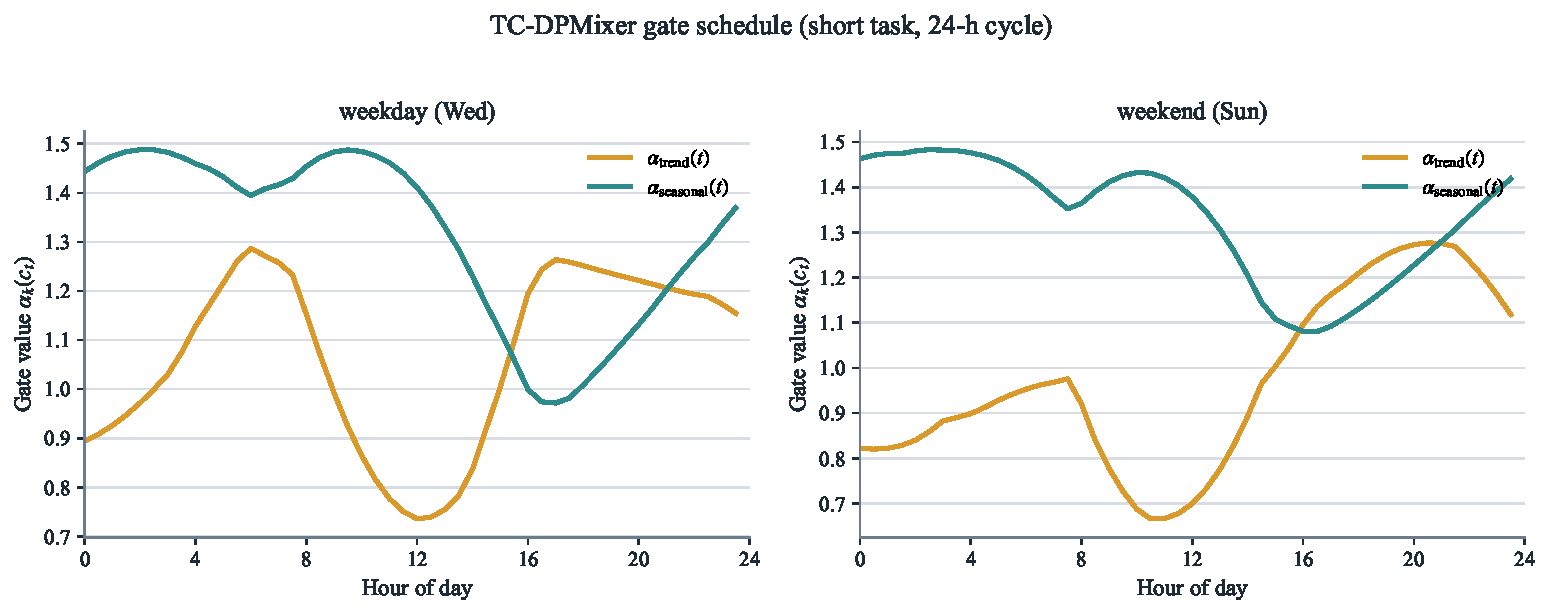
\includegraphics[width=0.85\linewidth]{figures/fig_gate_policy.pdf}
  \caption{\textbf{Calendar-conditioned gate schedule.} Plotted for
    TC-DLinear, a 2-gate variant of our calendar-routed mixers, as a
    clean illustration of the routing mechanism; the same
    $2\sigma(\mathrm{MLP}(c_{t}))$ gating appears in TC-DPMixer with
    four gates rather than two. A $\pm 10\,^{\circ}$C perturbation
    of outdoor temperature leaves the curve unchanged because
    temperature is not part of the gate's input.}
  \label{fig:gate}
\end{figure}

\paragraph{Three of four DPMixer branches are removable.}
Table~\ref{tab:ablation} reports a paired Wilcoxon test over the
3{,}829 short-task test windows. Removing the persistence anchor,
the target decomposition, or the channel mixer each produces a
small significant MAE drop. Removing the time-mixer branch is the
only edit whose effect cannot be distinguished from zero. Keeping
the persistence anchor alone is significantly worse. Read together,
the table localises the working part of DPMixer to a single learned
branch (the time mixer) plus the calendar gate; the other three
additive branches do not earn their parameters on this dataset.

\begin{table}[h]
  \centering
  \small
  \caption{Branch ablation against full DPMixer (MAE 35.96 Wh, 3829 test
    windows). $\Delta$\,MAE is the change after removing the named
    component. Significance is a paired Wilcoxon signed-rank test.}
  \label{tab:ablation}
  \begin{tabular}{lcc}
    \toprule
    Variant & $\Delta$\,MAE (Wh) & Wilcoxon \\
    \midrule
    Full DPMixer (ref.)        & $0$       & --      \\
    $-$ persistence anchor     & $-0.43$   & sig.\ better \\
    $-$ target decomposition   & $-0.66$   & sig.\ better \\
    $-$ channel mixer          & $-0.56$   & sig.\ better \\
    $-$ time mixer             & $+0.24$   & n.s.    \\
    Only persistence           & $+2.28$   & sig.\ worse \\
    \bottomrule
  \end{tabular}
\end{table}

\paragraph{A 116K minimal variant beats the 187K full model by 2.7 Wh/h on weekly.}
The ablation suggests a simpler model: persistence anchor, time-mixer
branch, calendar gate. We trained this configuration as Minimal-A
(Figure~\ref{fig:minimal}). On the weekly task it reached
$211.73 \pm 0.92$\,Wh/h at 116K parameters --- 2.71\,Wh/h below the
187K full TC-DPMixer ($214.44 \pm 0.75$) and 38\,\% smaller. Removing
the gate from the same configuration (Minimal-B) brings weekly MAE
back up to $214.83 \pm 0.50$, the full-model level. The gate, not
the depth of the additive backbone, accounts for the gain.

\begin{figure}[h]
  \centering
  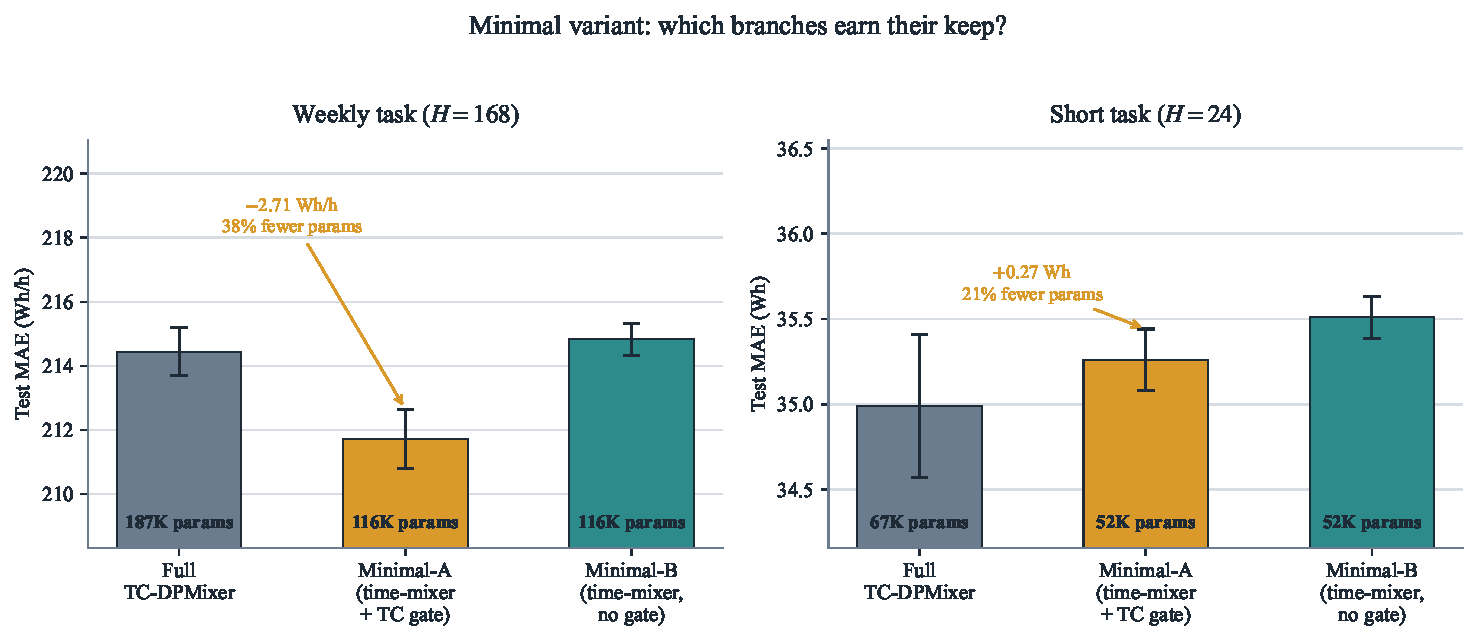
\includegraphics[width=0.95\linewidth]{figures/fig_minimal.pdf}
  \caption{\textbf{Minimal-variant ablation, 5 seeds, mean $\pm$ std.}
    On the weekly task (left), keeping only the persistence anchor, the
    time-mixer branch, and the TC gate (Minimal-A) lowers MAE by
    2.71 Wh/h while using 38\,\% fewer parameters than the full
    four-branch model. Removing the gate (Minimal-B) reverts the gain.
    The short task (right) is within noise across the three variants.}
  \label{fig:minimal}
\end{figure}

\paragraph{TC-DPMixer wins all four chronological folds on the weekly task.}
Sliding the chronological cut from 55\,\% to 70\,\% train ratio gives
four block-CV folds (Figure~\ref{fig:blockcv}). TC-DPMixer is the
lowest of the three models on every weekly fold; the per-fold gaps
over iTransformer are 10.9, 6.3, 13.3, and 5.9\,Wh/h. The short
task reverses on every fold, with iTransformer 0.85\,Wh ahead on
average. Both rankings mirror the headline split.
Table~\ref{tab:blockcv} in the supplementary material gives the
full per-fold numbers.

\begin{figure}[h]
  \centering
  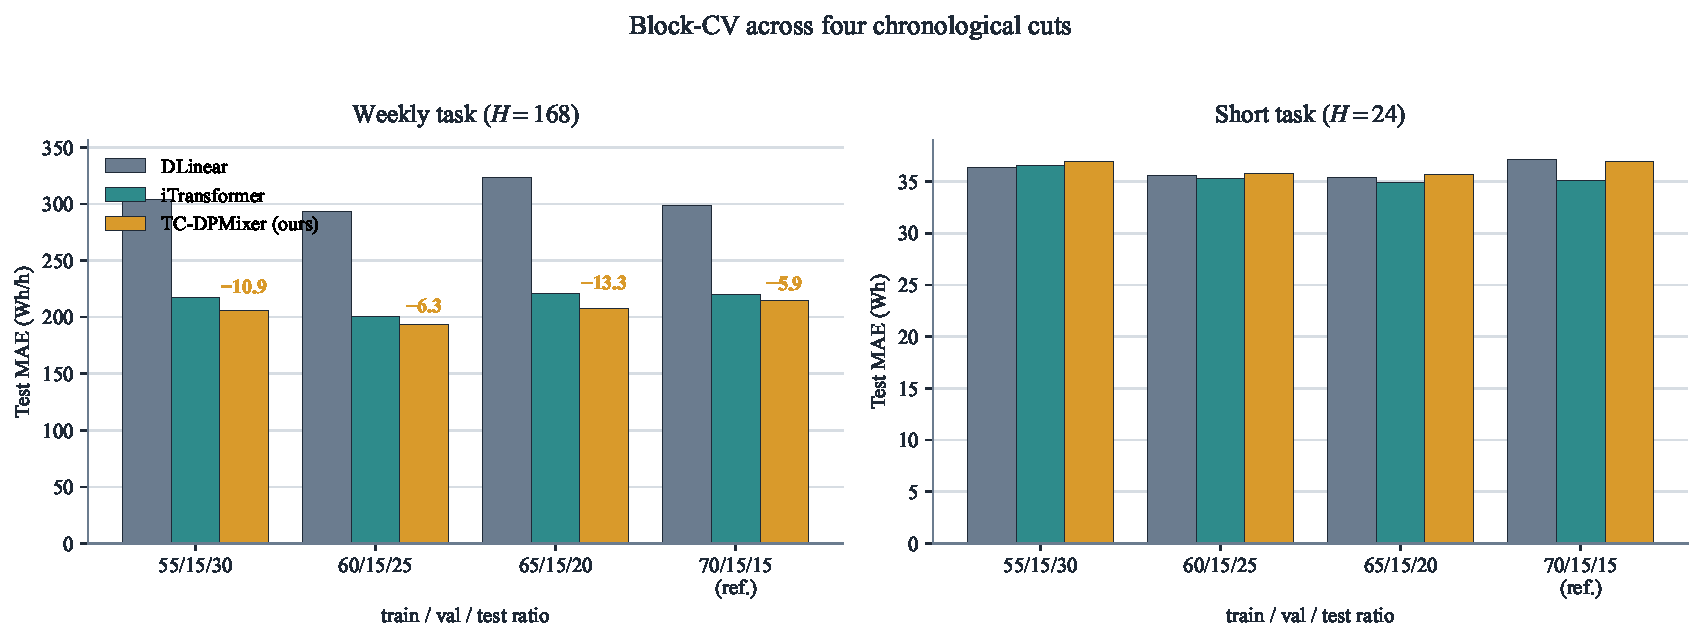
\includegraphics[width=0.95\linewidth]{figures/fig_block_cv.pdf}
  \caption{\textbf{Block-CV across four chronological cuts.}
    On the weekly task (left), TC-DPMixer attains the lowest MAE on
    every cut; per-fold gaps over iTransformer range from 5.9 to
    13.3 Wh/h. On the short task (right), the three models cluster
    tightly and iTransformer wins each fold.}
  \label{fig:blockcv}
\end{figure}

\paragraph{Self-history and hour-of-day dominate permutation importance.}
Permuting the appliance channel in TC-DPMixer's input raises test MAE
by 7.35\,Wh. Permuting \texttt{hour\_cos} raises it by 3.72. Permuting
outdoor temperature raises it by 0.06. Weather sits in the input as
context, not as a primary driver.

\section{Discussion}
\label{sec:discussion}

Three results converge on the same point. The learned 24-hour gate
schedule in Figure~\ref{fig:gate} is a non-trivial function of clock
time: the gate is doing work. The paired-Wilcoxon ablation in
Table~\ref{tab:ablation} says that among the four branches only
removing the time-mixer leaves accuracy statistically unchanged;
the other three branches can be dropped at no cost. The minimal
variant in Figure~\ref{fig:minimal} carries this finding to its
limit and reaches lower MAE than the full model at 38\,\% fewer
parameters. Read together, the three pieces of evidence point at one
mechanism: the calendar gate routes most of the load onto a single
inductive-bias branch (the time mixer), and that routing is what
the rest of this paper is reporting.

The horizon split is consistent with the same picture. The weekly
task is dominated by hour-of-day and weekday structure --- exactly
the signal the calendar gate encodes --- and TC-DPMixer leads on
every block-CV fold (Table~\ref{tab:blockcv}). The short task is
dominated by appliance inertia, on which the calendar gate carries
no information; iTransformer's cross-channel attention reaches a
0.84\,Wh advantage there.

The interpretability claim in this paper is scoped to the gate.
The gate output is a deterministic function of clock time, so it
cannot respond to weather or to load history. The rest of the
network still reads weather through the channel mixer, and we make
no claim about the full model's sensitivity to weather perturbations.

The work has clear limits. One dataset, one household, one climate,
4.5 months. The paired Wilcoxon $p{=}0.0625$ is at the $n{=}5$
exact-test floor: formal significance at $\alpha{=}0.05$ is out of
reach, and the bootstrap CI is what we lean on.

\section{Conclusion}
\label{sec:conclusion}

A 116K-parameter mixer with a calendar-conditioned gate reached
$211.73 \pm 0.92$\,Wh/h on the weekly task of UCI Appliances Energy,
below the 187K full TC-DPMixer and the 440K iTransformer in our
five-seed run. The setup is one household over 4.5 months. Whether
the learned 24-hour routing schedule transfers to a different building
is the question we did not answer here.

% =====================================================================
%   SUPPLEMENTARY INFORMATION
% =====================================================================
\appendix

\begin{center}
  \vspace{1em}
  \rule{0.6\linewidth}{0.4pt}\\[0.6em]
  {\Large\bfseries Supplementary Information}\\[0.4em]
  \rule{0.6\linewidth}{0.4pt}
  \vspace{1em}
\end{center}

\section{Related work}
\label{si:related}

\paragraph{Linear and decomposition baselines.}
DLinear and NLinear \citep{dlinear} showed that a single linear layer
on a trend--seasonal decomposition matches or beats deeper Transformer
forecasters on many long-horizon benchmarks. N-BEATS \citep{nbeats}
reaches similar conclusions with stacks of fully connected residual
blocks. These models are cheap and easy to audit but treat all
horizons identically; on weekly-scale household data the relative
importance of trend, season, and exogenous channels varies across
the day.

\paragraph{Mixer architectures.}
TSMixer \citep{tsmixer} and TimeMixer \citep{timemixer} introduce
time-mixing and channel-mixing MLPs as a transformer alternative.
PatchTST \citep{patchtst} and iTransformer \citep{itransformer} keep
self-attention but transpose its axis to model channels as tokens.
These models improve accuracy but spend parameter count and inference
cost to do so, and their attention maps over channels do not give the
operator a 24-hour schedule to sanity-check.

\paragraph{Routed mixtures.}
Mixture-of-Linear-Experts (MoLE) \citep{mole} routes linear
forecasters through a softmax gate. We adopt the routing form but
apply it to heterogeneous inductive-bias branches rather than
homogeneous linear experts, and we condition the gate on calendar
features only so its policy is a fixed 24-hour curve. NILM
sequence-to-point work \citep{nilm} motivates our use of the
appliance channel as the primary target.


\section{Implementation details}
\label{si:impl}

\paragraph{Branches.}
The target-decomposition branch uses a DLinear-style 25-point moving-
average kernel; trend and seasonal projections are both
\texttt{Linear(seq\_len $\to$ pred\_len)}. The channel mixer reads the
last timestep across all $C$ feature channels, passes it through two
MLP-Mixer blocks (hidden dim $128$, dropout $0.1$), and projects to
pred\_len. The time mixer applies the same MLP-Mixer pair along the
$L$ axis on the target channel only (hidden dim $128$, dropout $0.1$),
then projects to pred\_len.

\paragraph{Calendar gate.}
The gate MLP takes the 6-dim calendar feature vector
(hour\_sin/cos, weekday\_sin/cos, weekend\_flag, NSM) at the
last input step and outputs four branch weights via
$\sigma(\mathrm{MLP}(c_t)) \cdot 2$, giving weights in
$[0, 2]^{4}$. The MLP is
$\mathrm{Linear}(6 \to 16) \to \mathrm{ReLU} \to \mathrm{Linear}(16 \to 4)$
with the output layer initialised to zero so that the initial
branch weights equal one.

\paragraph{Training.}
All models train with Adam ($\eta=10^{-3}$, weight decay $10^{-4}$),
$L_1$ loss on a $\log(1+y)$-transformed target, batch size 64, and
early stopping with patience 10. We use chronological 70/15/15 splits
on the headline runs and 55/15/30, 60/15/25, 65/15/20, 70/15/15 splits
on the block-CV runs. Five seeds (\texttt{42--46}) are used for every
mean$\pm$std reported in the main paper. No hyperparameters were
tuned on the test split.

\paragraph{Hardware.}
The latency benchmark in Table~\ref{tab:lat} ran on a single
NVIDIA RTX 6000 Ada GPU under PyTorch 2.4.0+cu121 in eager mode,
with 100 warm-up forwards and 1{,}000 timed forwards per
configuration.


\section{Supplementary tables}
\label{si:tables}

\begin{table}[h]
\centering
\caption{Block-CV across four chronological cuts on the weekly task
(Wh/h). The 70/15/15 row is the headline split.}
\label{tab:blockcv}
\small
\begin{tabular}{lccc}
\toprule
train/val/test & DLinear & iTransformer & TC-DPMixer \\
\midrule
55 / 15 / 30 & 304.24 & 217.17 & \textbf{206.27} \\
60 / 15 / 25 & 293.45 & 200.10 & \textbf{193.78} \\
65 / 15 / 20 & 323.70 & 220.45 & \textbf{207.17} \\
70 / 15 / 15 & 299.00 & 220.18 & \textbf{214.24} \\
\midrule
Mean         & 305.10 & 214.48 & \textbf{205.37} \\
Std (4 folds)& 13.16  & 9.70   & 8.51 \\
\bottomrule
\end{tabular}
\end{table}

\begin{table}[h]
\centering
\caption{Paired-seed comparison (5 seeds, weekly task).
Source: \texttt{results/paired\_test\_weekly.json}.}
\label{tab:paired}
\small
\begin{tabular}{lc}
\toprule
Quantity & Value \\
\midrule
iTransformer mean MAE             & $219.91 \pm 2.42$ \\
TC-DPMixer mean MAE               & $214.44 \pm 0.75$ \\
Mean paired difference (TC$-$iTrans) & $-5.47$ \\
sd of paired difference              & $1.91$ \\
95\,\% bootstrap CI (10{,}000 resamples) & $[-6.93,\ -4.11]$ \\
Paired Cohen's $d$                & $-2.87$ \\
Wilcoxon signed-rank $W$          & $0$ \\
Wilcoxon two-sided $p$ (exact)    & $0.0625$ (= $n{=}5$ floor) \\
\bottomrule
\end{tabular}
\end{table}

\begin{table}[h]
\centering
\caption{Inference latency (ms / window) on the weekly task.
Hardware: NVIDIA RTX 6000 Ada, PyTorch 2.4.0+cu121, eager mode,
100 warm-up + 1{,}000 timed forwards. Source:
\texttt{results/latency\_weekly.csv}.}
\label{tab:lat}
\small
\begin{tabular}{lcccc}
\toprule
Model        & bs $=1$ mean & bs $=1$ p99 & bs $=32$ mean & Params \\
\midrule
DLinear      & 0.147 & 0.170 & 0.004 & 57K  \\
iTransformer & 0.336 & 0.465 & 0.187 & 440K \\
PatchTST     & 0.337 & 0.452 & 0.031 & 447K \\
DPMixer      & 0.361 & 0.541 & 0.012 & 187K \\
TC-DPMixer   & 0.380 & 0.453 & 0.014 & 187K \\
\bottomrule
\end{tabular}
\end{table}

\paragraph{Permutation importance, full table.}
Top contributing channels by $\Delta$\,MAE on TC-DPMixer
(short task, single seed):
Appliances $+7.35$, hour\_cos $+3.72$, Tdewpoint $+1.54$,
hour\_sin $+1.16$, T6 $+0.99$, RH\_2 $+0.83$, T2 $+0.69$;
outdoor temperature $T_\text{out}$ contributes $+0.06$.
Source: \texttt{results/permutation\_importance.csv}.


\section{Additional ablations}
\label{si:additional}

This appendix consolidates ablations on the short-horizon task that
support the headline recipe (\texttt{no\_rv + time + log\_target},
$L_1$ loss).

\paragraph{Feature engineering.}
Using only the target's own history is competitive with using all 26
sensors; adding time encodings and a $\log(1+y)$ target transform
yields the strongest configuration.

\begin{table}[h]
\centering
\small
\caption{Feature ablation (short task, test MAE in Wh).}
\label{tab:feat}
\begin{tabular}{lrrr}
\toprule
Configuration & LSTM & DLinear & $n_{\text{feat}}$ \\
\midrule
\texttt{target\_only}                           & 40.3 & 44.7 & 1  \\
\texttt{target\_time}                           & 40.5 & 43.5 & 7  \\
\texttt{target\_indoor}                         & 45.5 & 49.3 & 19 \\
\texttt{no\_rv}                                 & 51.5 & 46.9 & 26 \\
\texttt{all}                                    & 47.8 & 52.2 & 28 \\
\textbf{\texttt{no\_rv + time + log\_target}}   & \textbf{39.9} & \textbf{37.9} & 32 \\
\texttt{all + time + log\_target}               & 46.2 & 41.4 & 34 \\
\bottomrule
\end{tabular}
\end{table}

\paragraph{Training-loss ablation.}
Switching MSE to $L_1$ reduces MAE by 5--20 Wh on every architecture
on the short task; this is the metric--objective alignment that
explains the milestone's MLP-vs-Persistence anomaly.

\begin{table}[h]
\centering
\small
\caption{Loss-function comparison (short task, test MAE in Wh).}
\label{tab:loss}
\begin{tabular}{lrrrr}
\toprule
Loss & MLP & LSTM & DLinear & PatchTST \\
\midrule
MSE      & 59.3          & 43.8          & 46.9          & 64.0 \\
$L_1$    & \textbf{39.2} & \textbf{41.2} & \textbf{37.3} & \textbf{44.8} \\
Huber    & 45.5          & 38.7          & 40.9          & 46.1 \\
SmoothL1 & 52.5          & 41.6          & 39.7          & 46.1 \\
\bottomrule
\end{tabular}
\end{table}

\paragraph{Forecast-horizon sweep.}
Persistence is unbeatable at $H{=}6$ (1\,h); deep models overtake
from $H{=}12$ onwards; DLinear stays remarkably flat across horizons.

\begin{table}[h]
\centering
\small
\caption{Forecast horizon sweep (test MAE in Wh).}
\label{tab:hor}
\begin{tabular}{lrrrr}
\toprule
Horizon (h) & Persistence & LSTM & DLinear & PatchTST \\
\midrule
1 (H=6)   & \textbf{38.2} & 40.4 & 39.8          & 46.3 \\
2 (H=12)  & 42.5          & 46.2 & \textbf{43.3} & 55.5 \\
4 (H=24)  & 48.9          & 45.7 & 46.9          & 64.0 \\
8 (H=48)  & 56.0          & 61.8 & \textbf{56.6} & 60.0 \\
16 (H=96) & 62.1          & 65.3 & \textbf{52.8} & 55.5 \\
\bottomrule
\end{tabular}
\end{table}

\paragraph{Input-corruption robustness.}
Standardised-input Gaussian noise barely moves the deep models;
random feature masking is far more damaging. Persistence is immune
to feature masking because it never uses non-target features.

\begin{table}[h]
\centering
\small
\caption{Robustness under inference-time corruption (test MAE in Wh).}
\label{tab:corr}
\begin{tabular}{lrrrrr}
\toprule
Model & Clean & $\sigma{=}0.1$ & $\sigma{=}0.3$ & Mask 20\% & Mask 40\% \\
\midrule
Persistence & 48.9          & 51.2          & 61.1          & 48.9          & 48.9          \\
MLP         & 48.6          & 48.6          & 48.8          & 61.4          & 66.6          \\
LSTM        & \textbf{41.7} & \textbf{41.7} & \textbf{41.8} & \textbf{47.6} & \textbf{50.8} \\
DLinear     & 53.1          & 53.1          & 53.9          & 59.7          & 62.1          \\
PatchTST    & 56.3          & 56.2          & 56.0          & 62.5          & 64.8          \\
\bottomrule
\end{tabular}
\end{table}


\section*{LLM Usage}
Claude Opus 4.7 (Anthropic) was used throughout this project as a
coding and writing assistant. Its specific roles were: (i) drafting and
debugging Python experiment scripts (training loops, ablation harnesses,
figure generation), each of which the author read, executed, and
verified before any output was cited; (ii) drafting and polishing
English prose in this report; and (iii) scaffolding LaTeX tables, figure
includes, and bibliography entries. The author designed the study,
chose every hyperparameter, ran every reported experiment, verified
each cited number against the corresponding CSV in the project
repository, and authored all interpretations and claims. Any error
that may have originated in LLM output remains the author's
responsibility.

\begin{thebibliography}{9}

\bibitem{candanedo2017}
L.\ M.\ Candanedo, V.\ Feldheim, and D.\ Deramaix.
\newblock Data driven prediction models of energy use of appliances in a
  low-energy house.
\newblock \emph{Energy and Buildings}, 140:81--97, 2017.

\bibitem{dlinear}
A.\ Zeng, M.\ Chen, L.\ Zhang, and Q.\ Xu.
\newblock Are transformers effective for time series forecasting?
\newblock In \emph{AAAI}, 2023.

\bibitem{tsmixer}
S.-A.\ Chen, C.-L.\ Li, N.\ Yoder, S.\ O.\ Arik, and T.\ Pfister.
\newblock TSMixer: An all-MLP architecture for time series forecasting.
\newblock \emph{Transactions on Machine Learning Research}, 2023.

\bibitem{timemixer}
S.\ Wang et al.
\newblock TimeMixer: Decomposable multiscale mixing for time series
  forecasting.
\newblock In \emph{ICLR}, 2024.

\bibitem{nbeats}
B.\ N.\ Oreshkin, D.\ Carpov, N.\ Chapados, and Y.\ Bengio.
\newblock N-BEATS: Neural basis expansion analysis for interpretable
  time series forecasting.
\newblock In \emph{ICLR}, 2020.

\bibitem{mole}
W.\ Ni et al.
\newblock Mixture-of-Linear-Experts for long-term time series
  forecasting.
\newblock In \emph{AISTATS}, 2024.

\bibitem{nilm}
C.\ Zhang, M.\ Zhong, Z.\ Wang, N.\ Goddard, and C.\ Sutton.
\newblock Sequence-to-point learning with neural networks for
  non-intrusive load monitoring.
\newblock In \emph{AAAI}, 2018.

\bibitem{patchtst}
Y.\ Nie, N.\ H.\ Nguyen, P.\ Sinthong, and J.\ Kalagnanam.
\newblock A time series is worth 64 words: Long-term forecasting with
  transformers.
\newblock In \emph{ICLR}, 2023.

\bibitem{itransformer}
Y.\ Liu et al.
\newblock iTransformer: Inverted transformers are effective for time
  series forecasting.
\newblock In \emph{ICLR}, 2024.

\end{thebibliography}

\end{document}
